%%%%%%%%%%%%%%%%%%%%%%%%%%%%%%%%
\section{Results}
%%%%%%%%%%%%%%%%%%%%%%%%%%%%%%%%
%
Research has shown that children with CI can attain spoken language skills similar to
those of their normal hearing peers after three to four years of device use (i.a., Bruijnzeel, Ziylan, Stegeman, Topsakal, \& Grolman, 2016; Dettman, Dowell, Choo, Arnott, Abrahams, Davis, Dornan, Leigh, Constantinescu, Cowan, \& Briggs, 2016; Geers, \& Nicholas,
2013; Wie et al., 2020). However, the population of children with CI is characterized by remarkable variation. On the one hand, variation relates to differences between individual children: while a considerable number of children with CI appear to catch up with their NH peers, some do not catch up at all (Duchesne, \& Marschark, 2019; Geers, Nicholas, Tobey, \& Davidson, 2016; Nicholas, \& Geers, 2007). On the other hand, variation also relates to differences between domains: some areas of speech and language appear to be more difficult to master than others (Duchesne, \& Marschark, 2019). For instance, Faes, Gillis, \& Gillis (2015) showed that in a group of children with CI acquiring Dutch, inflectional morphology and sentence length (as a proxy of syntagmatic development) were age-appropriate when the children were 7;0, but the former (and not the latter) was already age-appropriate at age 5;0. Moreover, the phonetics of the same children’s production of vowels was still significantly different from the vowels of their NH peers
at the age of 7;0 (Verhoeven, Hide, De Maeyer, Gillis, \& Gillis, 2016). Thus, although
children with CI start with an initial delay in spoken language, a quite significant group
eventually reaches age appropriate levels of linguistic functioning. But the individual
variation is also quite large: while some children do catch up with their normally hearing
peers, others do not achieve much language comprehension and production even after five years of device use (Barnard, Fisher, Johnson, Eisenberg, Wang, Quittner, Carson, \&
Niparko, 2015).



As to intelligibility, most studies found that CI children’s speech intelligibility is less
well developed than that of their NH peers (i.a., Castellanos, Kronenberger, Beer Henning, Colson, \& Pisoni, 2014; Chin, \& Kuhns, 2014; Freeman et al., 2017; Grandon et al., 2020). 
%
\begin{figure}
	\centering
	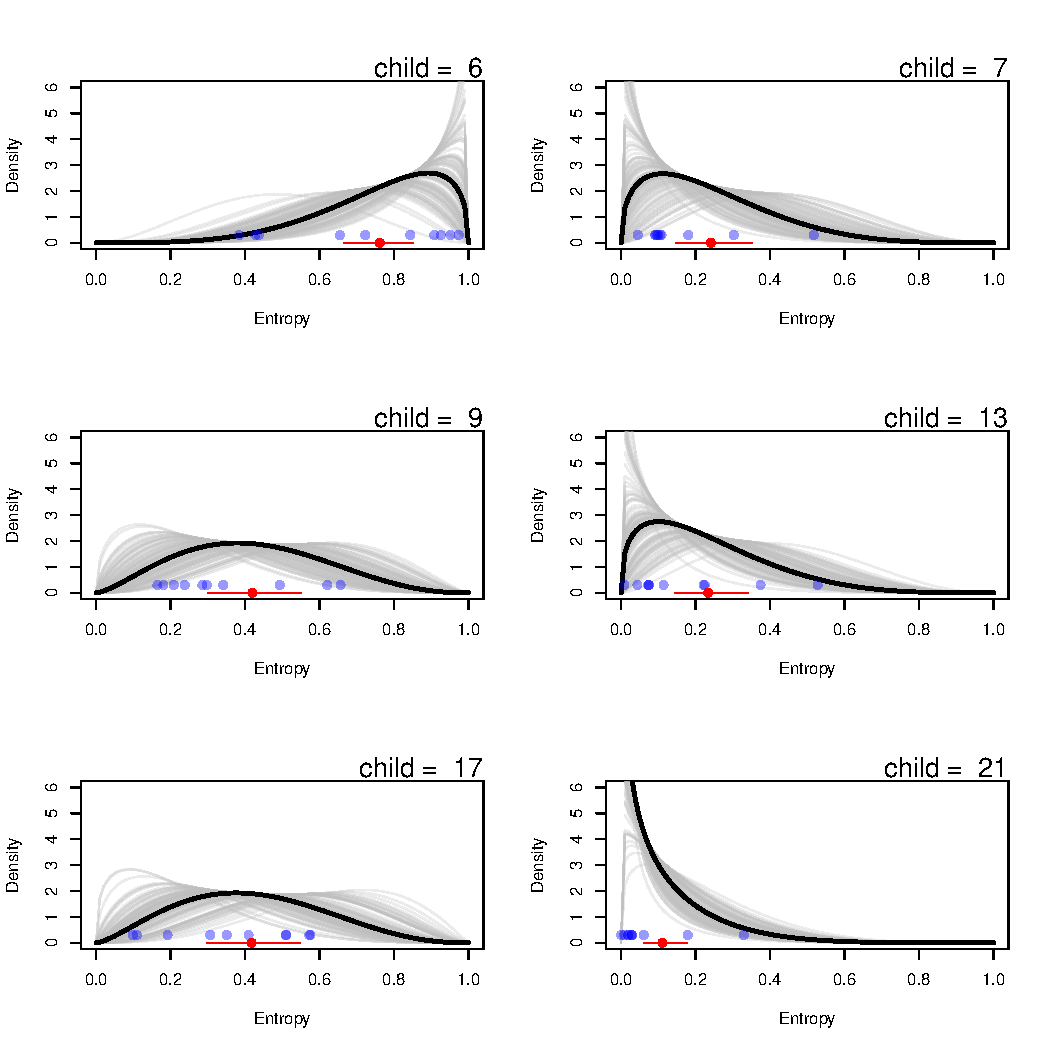
\includegraphics[width=0.5\linewidth]{posterior_predictive_real1.pdf}
	\caption[Posterior predictive: entropy replicates]{Posterior predictive: entropy replicates}
	\label{fig:predictive1}
\end{figure}
%
\begin{figure}
	\centering
	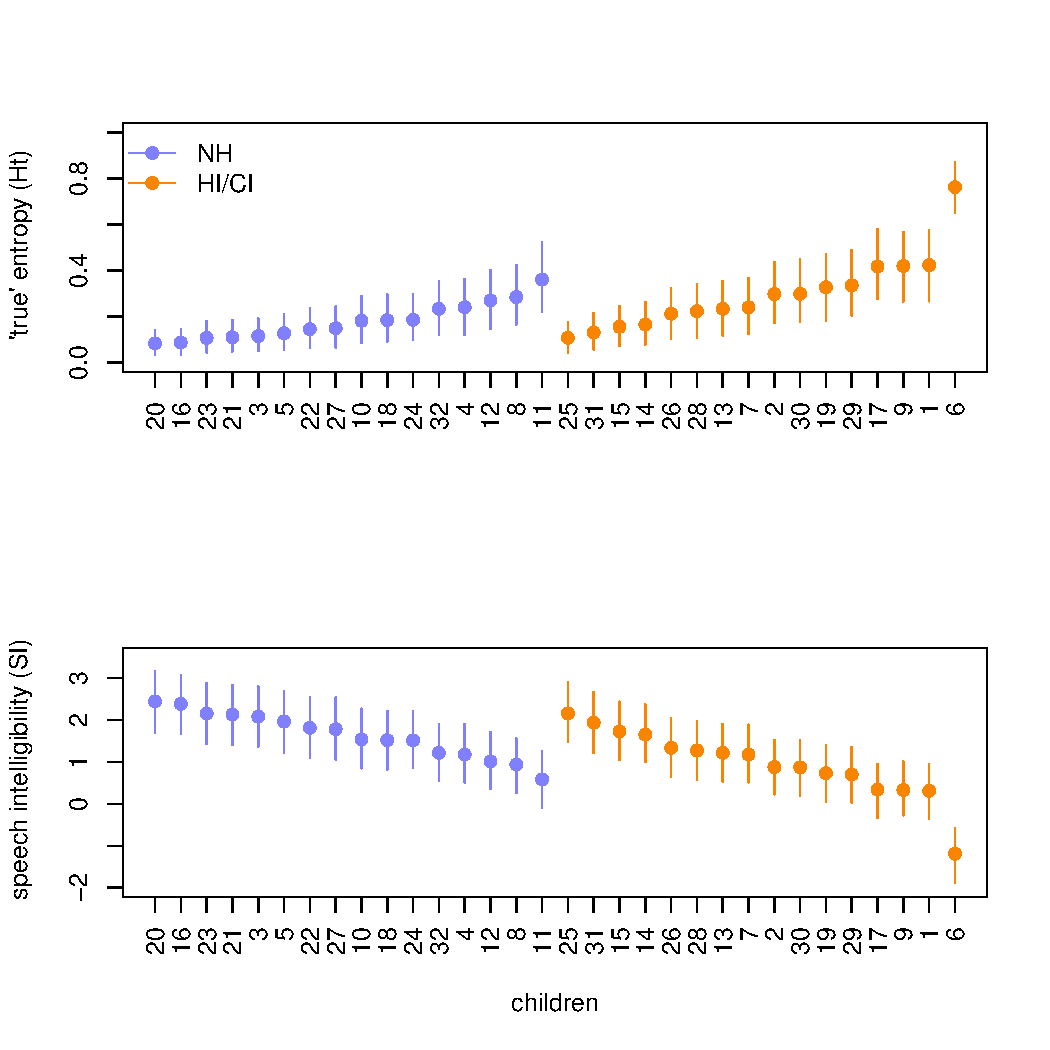
\includegraphics[width=0.5\linewidth]{posterior_predictive_real2.pdf}
	\caption[Posterior predictive: ``true'' entropy and intelligibility scales]{Posterior predictive: ``true" entropy and intelligibility scales}
	\label{fig:predictive2}
\end{figure}
%
\begin{figure}
	\centering
	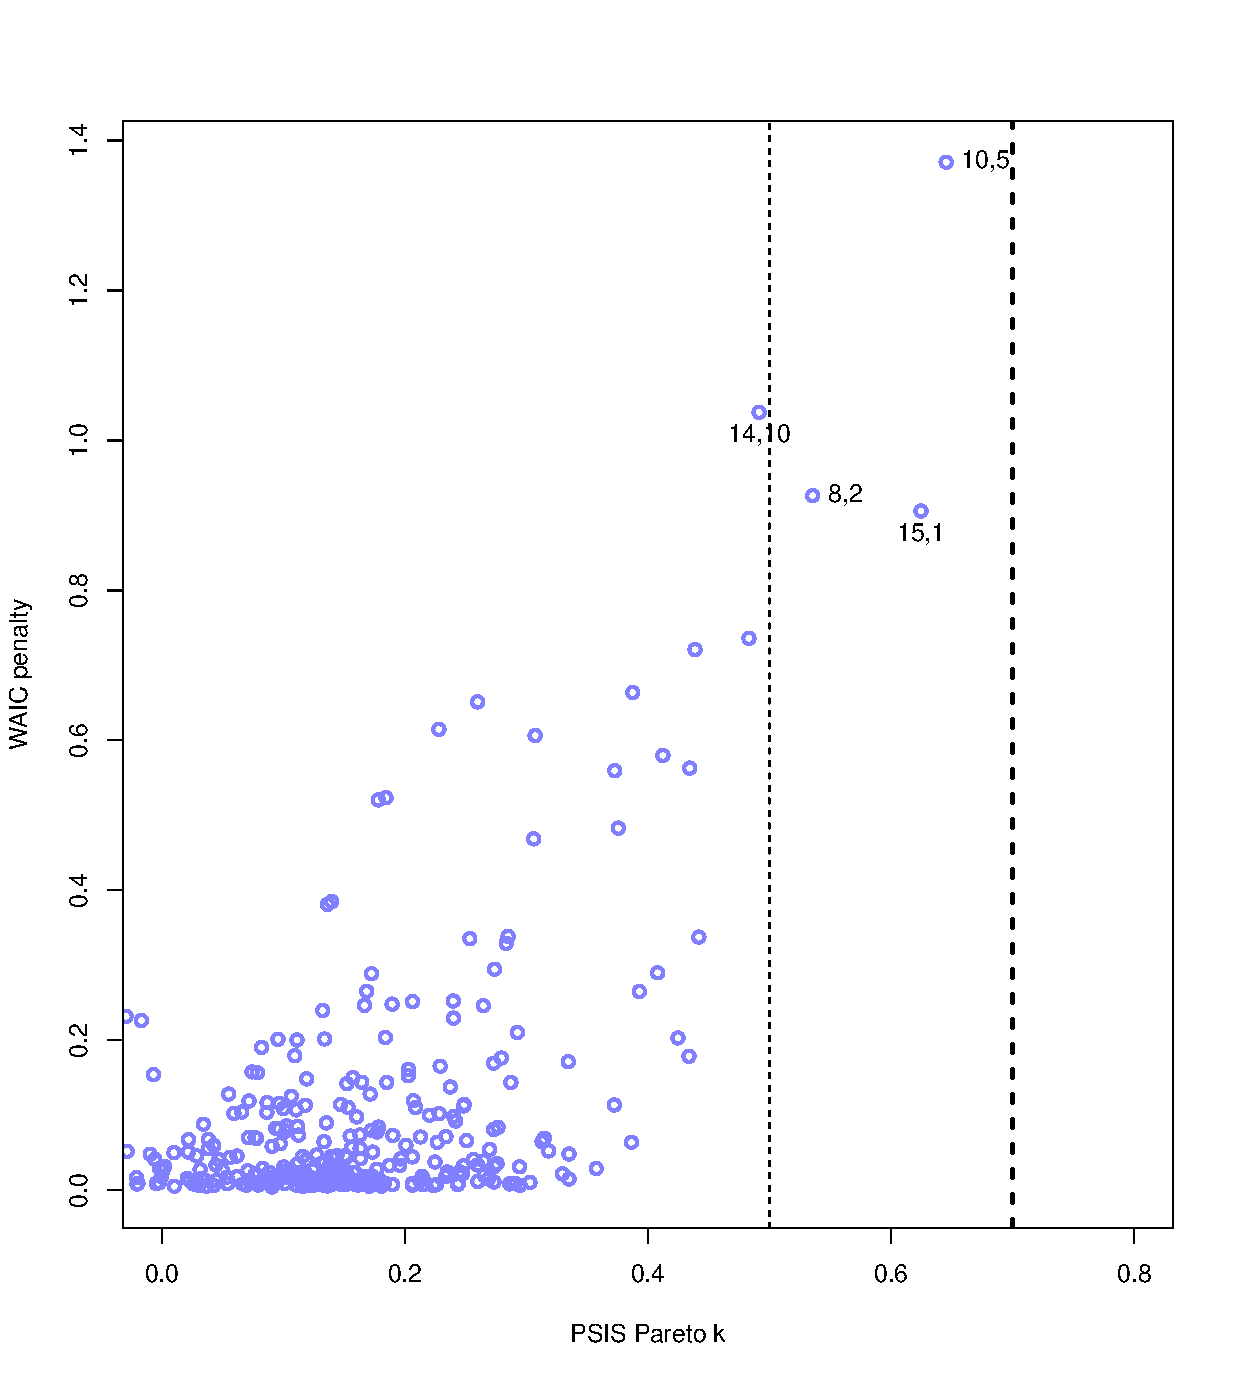
\includegraphics[width=0.5\linewidth]{outliers.pdf}
	\caption[Outlying observations]{Outlying observations}
	\label{fig:outliers}
\end{figure}
%
\begin{figure}
	\centering
	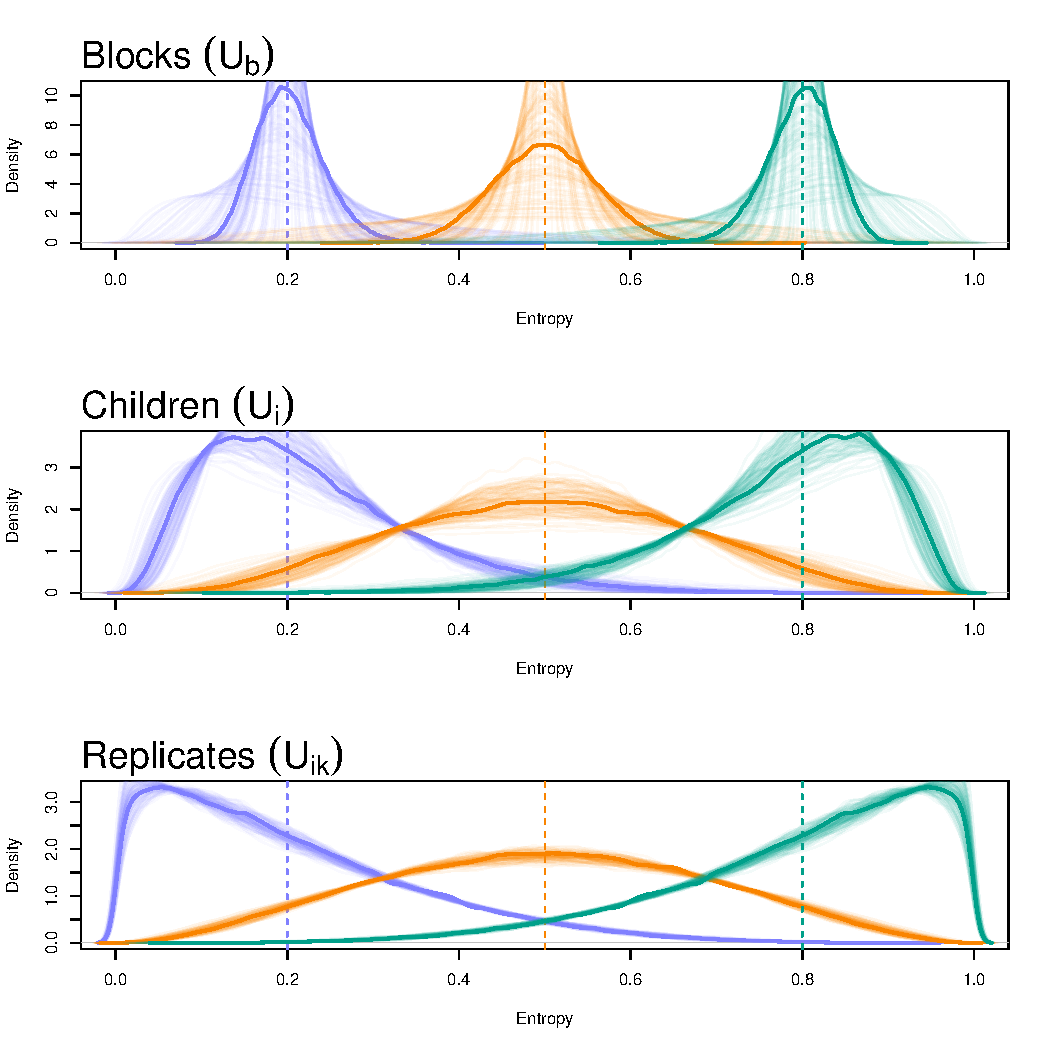
\includegraphics[width=0.5\linewidth]{variability_plot.pdf}
	\caption[Posterior predictive: levels of variability]{Posterior predictive: levels of variability}
	\label{fig:variability}
\end{figure}